\section{Section 3: Logistics Growth Model}
\subsection{Background}
\begin{frame}{Logistic growth}
    The \textbf{logistic growth model represents how populations change over time when resources imitated}.  The logistic model incorporates a carrying capacity—the maximum population size a specific environment can sustainably support.
\pause
\vfill
\textbf{Key Concepts}

\begin{itemize}
    \item \textbf{Carrying Capacity ($K$)}: A ceiling that limits population growth due to limited resources  (food, space, water, etc.)
    \pause
    \item \textbf{Intrinsic Growth Rate ($r$)}: The rate at which a population would grow if there were unlimited resources.
    \pause
    \item \textbf{S-Shaped Curve}: The logistic growth model plots as an S-shaped curve. Growth is initially exponential, then slows as it approaches the carrying capacity.
\end{itemize}

\end{frame}

\begin{frame}{Equation of logistic growth}
\footnotesize
Differential equation of logistic growth
\begin{equation*}
       \frac{dP}{dt} = rP\left(1 - \frac{P}{K}\right)
\end{equation*}
\pause
Iterative Form:
\begin{equation*}
 P(t_{i+1}) = P(t_i) + rP(t_i)\left(1 - \frac{P_t}{K}\right) \Delta t
\end{equation*}
\pause
Explicit solution
\begin{equation*}
P(t) = \frac{K}{1 + \left(\frac{K - P_0}{P_0} \right) e^{-rt}}
\end{equation*}
\pause
where 
\begin{itemize}
    \item $P(t_i)$ is the population at time $t_i$
    \pause
    \item $P_0$ is initial population
    \pause
    \item $r$ is the growth rate
    \pause
    \item $K$ is carrying capacity
    \pause
    \item $t$ is time, $\Delta t$ is the time step
\end{itemize}
\end{frame}


\begin{frame}[t]{Logistic growth of population over time}
\begin{center}
    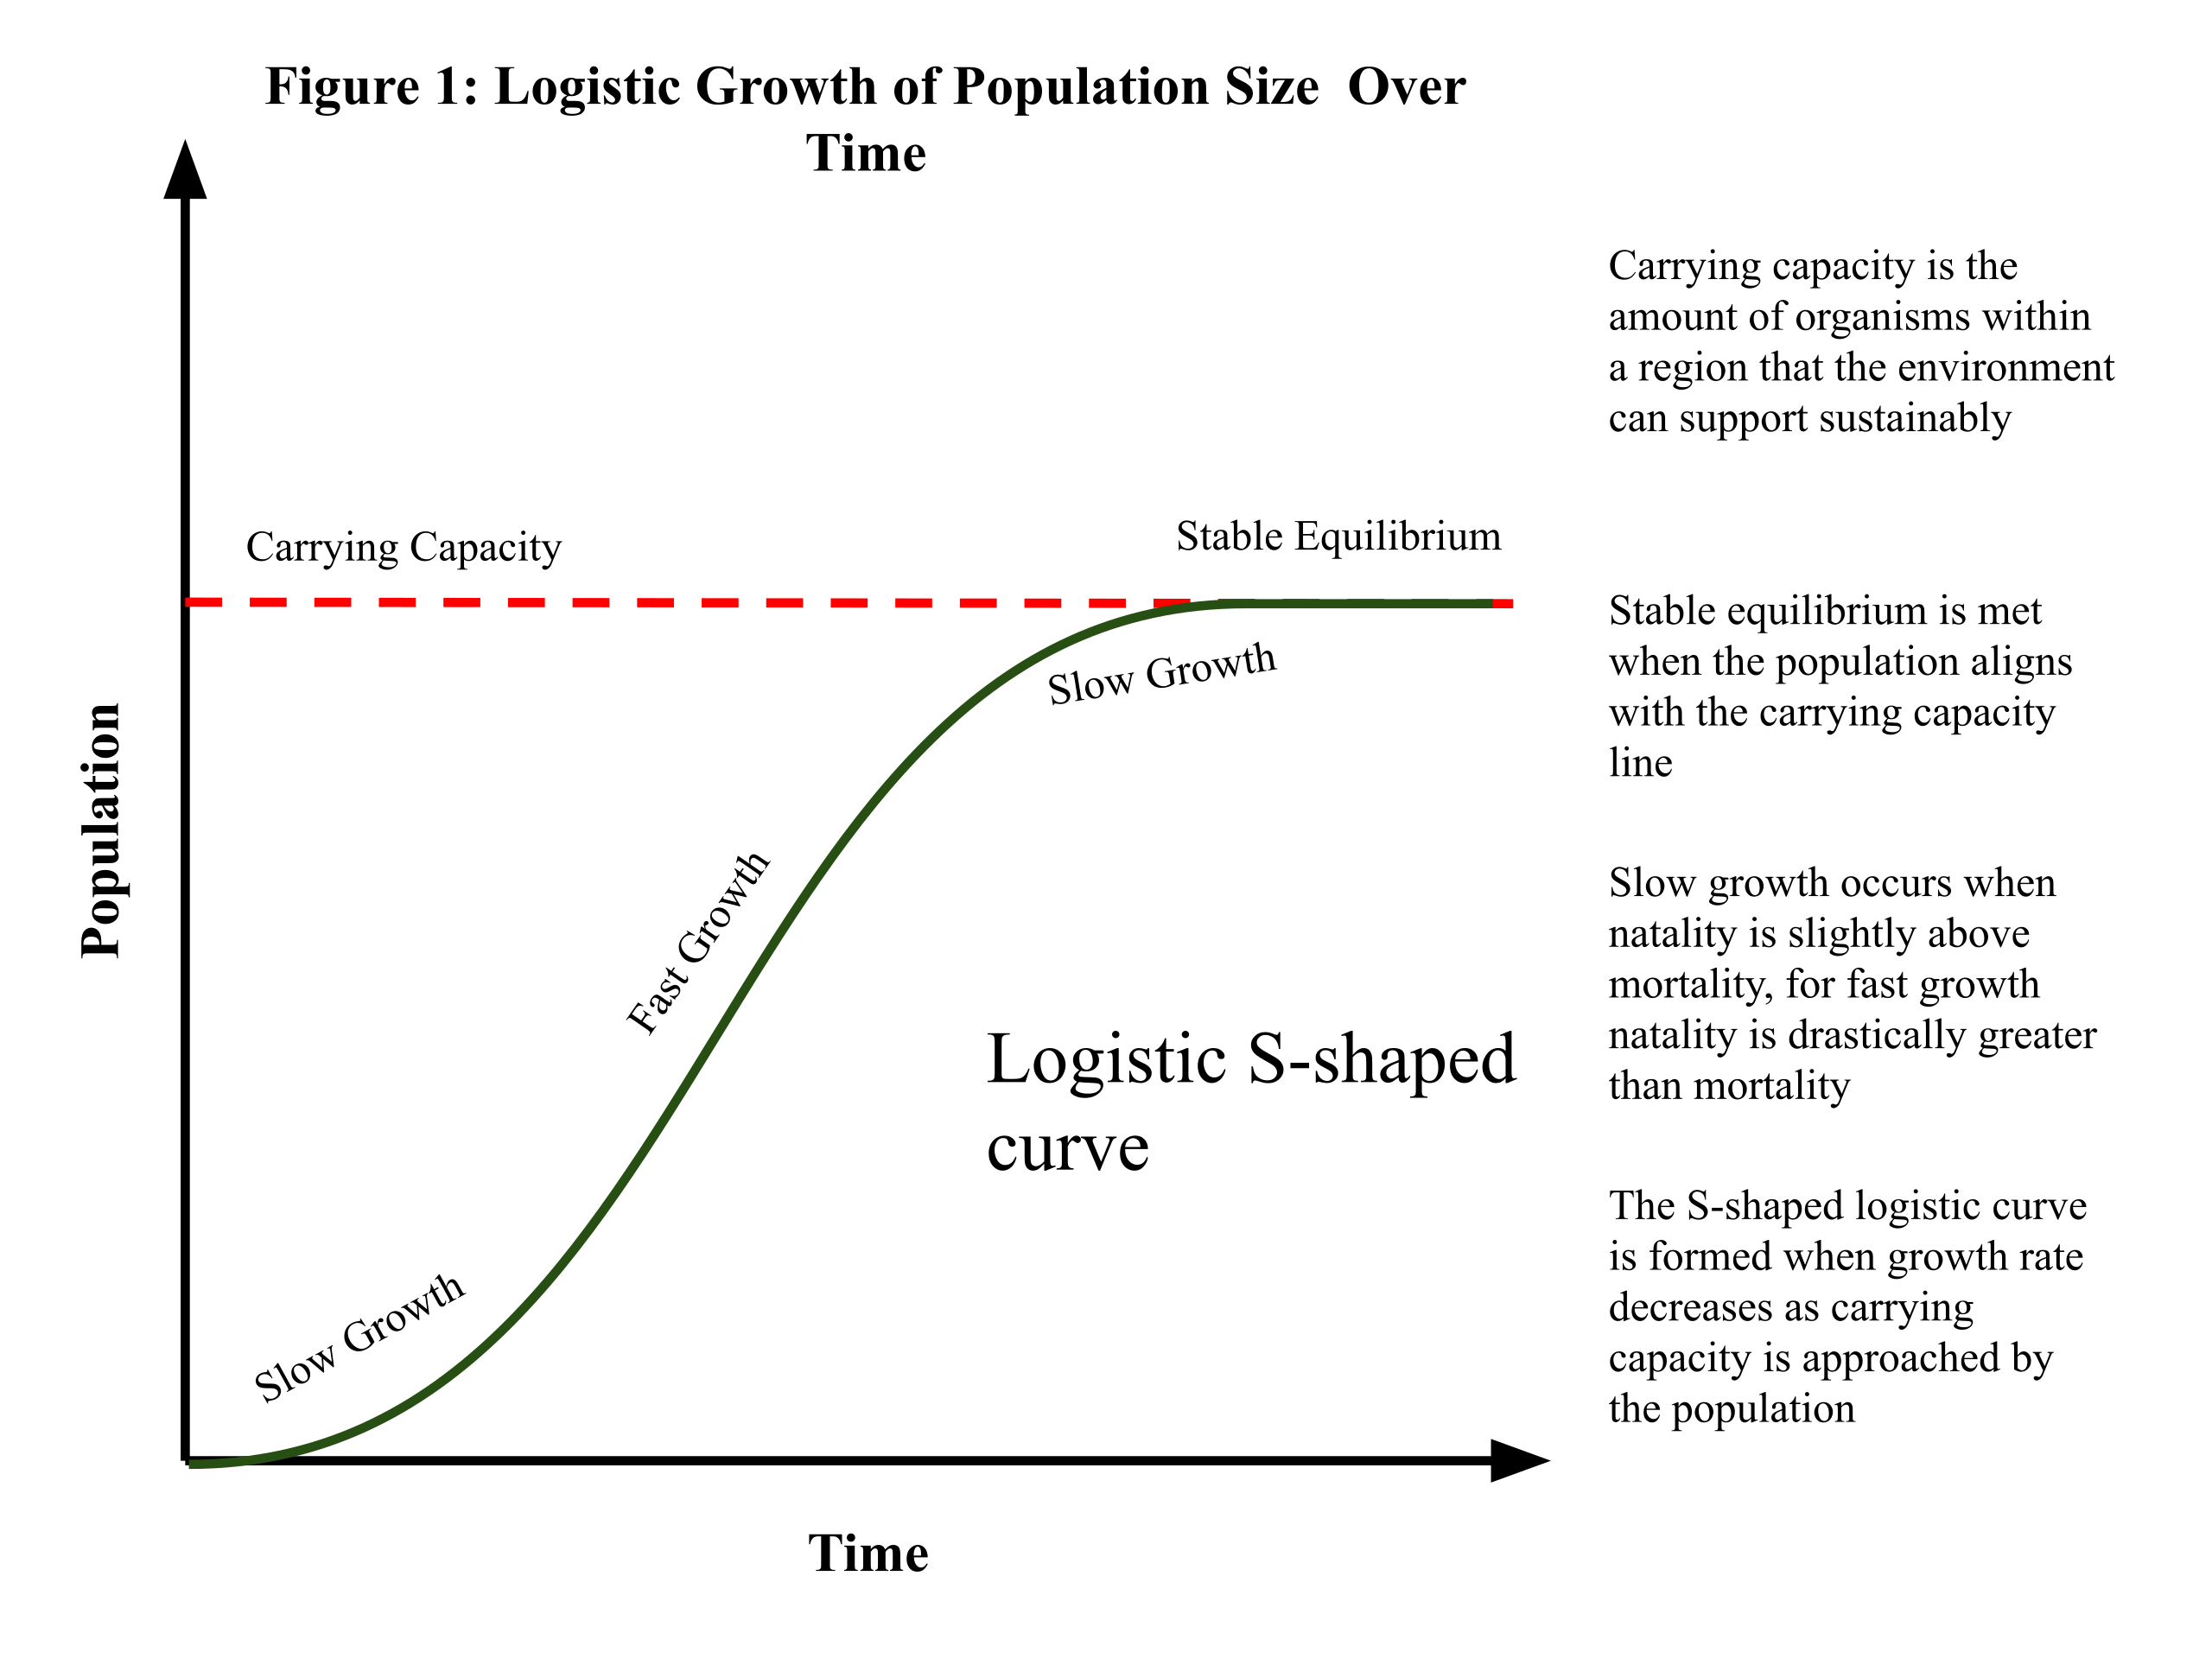
\includegraphics[scale = 0.11]{lesson_1/images/logistic_model_curve.png}
\end{center}
\end{frame}

\begin{frame}{Example --- French and English railway construction}
\small
    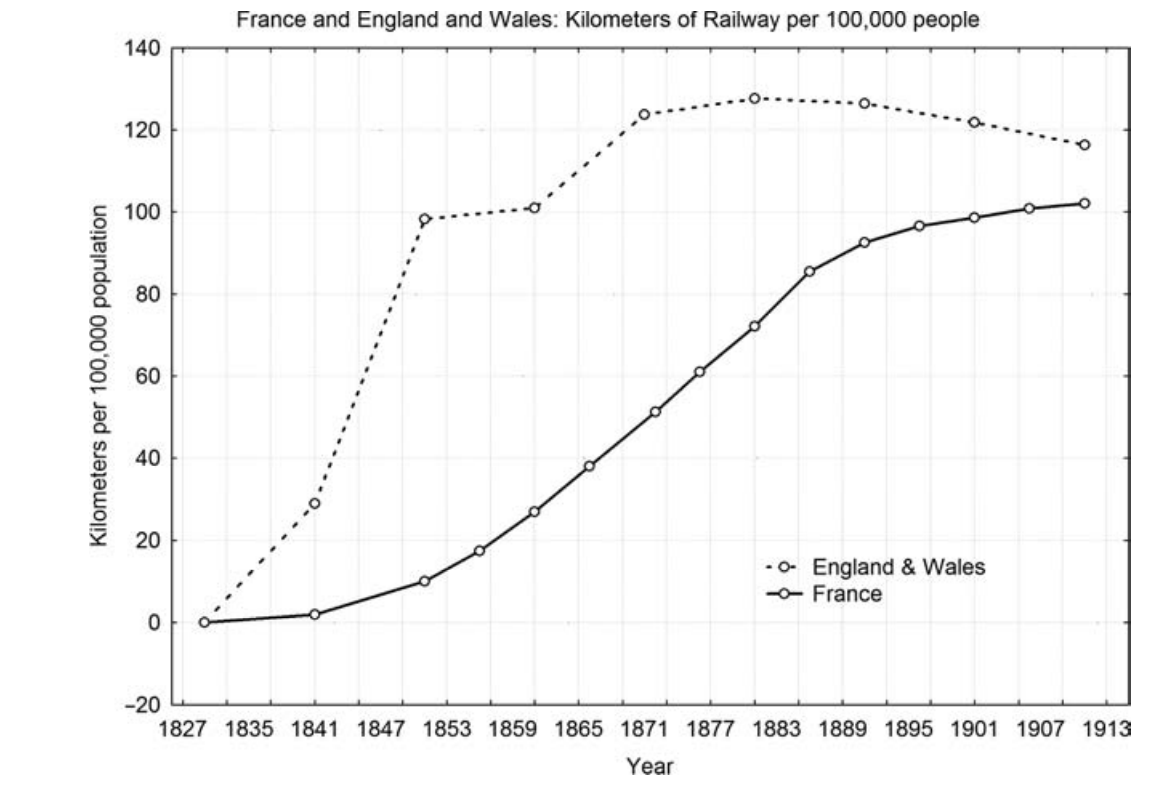
\includegraphics[scale = 0.3]{lesson_1/images/logistic_model_railroad_curve.png}
    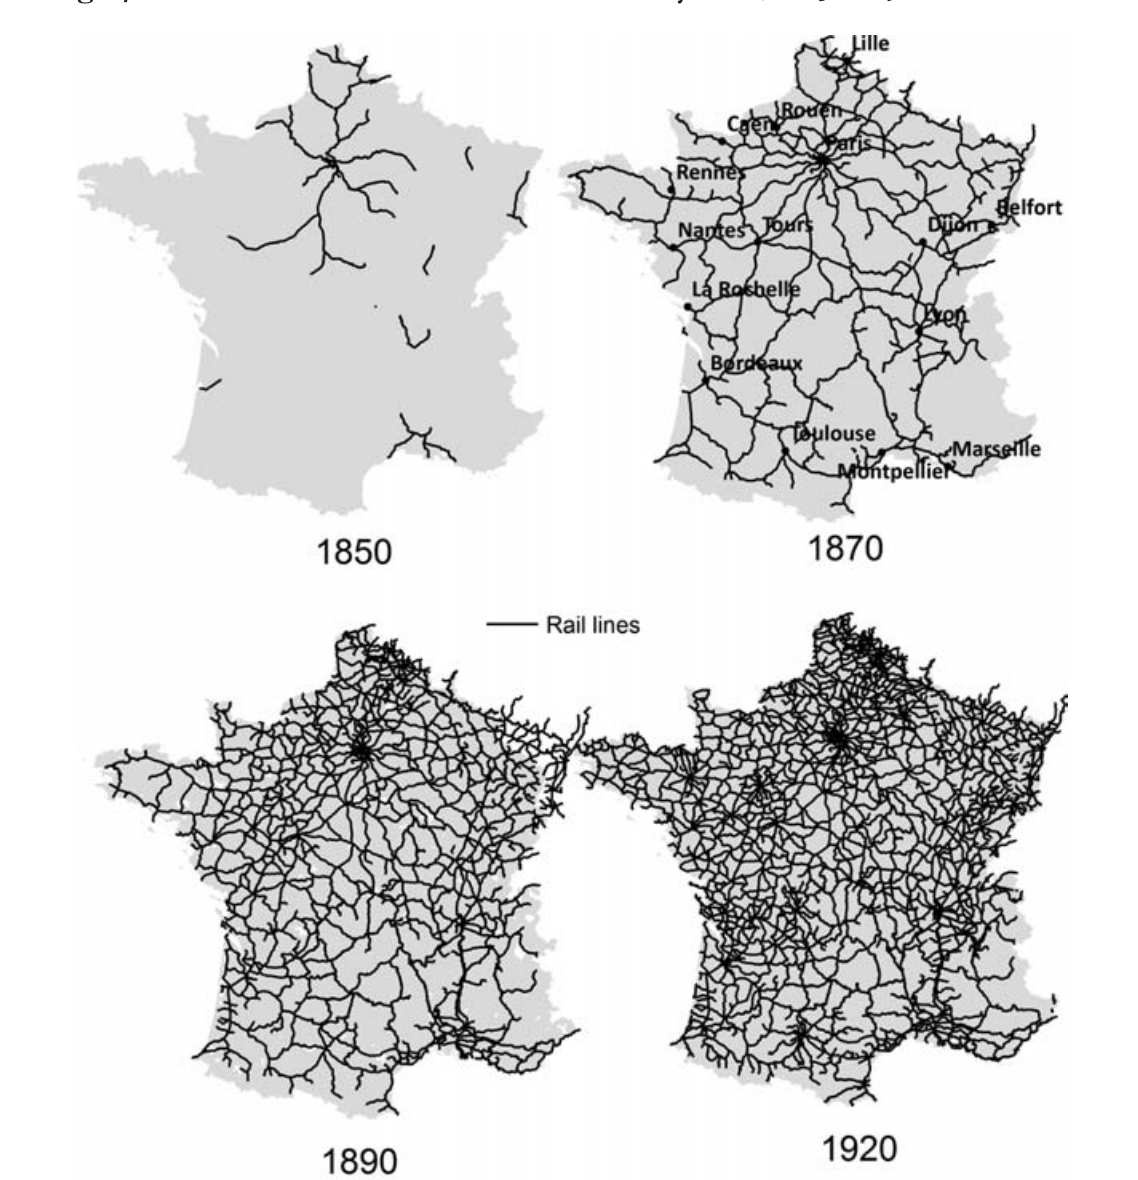
\includegraphics[scale = 0.2]{lesson_1/images/logistic_model_railroad.png}
    \pause
\textbf{Topics for discussion}
    \begin{itemize}
        \item Why do you think that the French railway construction follows logistic growth but English does not? 
        \pause
        \item How would you explain \textbf{carrying capacity} in the context of railroad construction?
        \pause
        \item What may affect carrying capacity for railways? Is the capacity it constant or dynamic? 
    \end{itemize}
\end{frame}


\begin{frame}{Closer look at logistic growth equation }
Differential equation of logistic growth
\begin{equation*}
       \frac{dP}{dt} = rP\left(1 - \frac{P}{K}\right)
\end{equation*}
\vfill
\textbf{Let’s explore the equation}
\begin{itemize}
    \item Try to figure out how  carrying capacity affects the population growth. Try different combinations of P an K. 
    \pause
    \item What are equilibria solutions where there is no population growth? 
\end{itemize}
\end{frame}

\begin{frame}{Derivation of Equilibrium Solutions:}
\small
To find equilibrium solutions, we set $\frac{dP}{dt} = 0$:
\begin{equation*}
   0 = rP \left(1 - \frac{P}{K}\right) 
\end{equation*}
    \pause
This equation is satisfied when either
\begin{itemize}
    \item  Population is zero \begin{equation*}
   P = 0
\end{equation*}
    \pause
\item Growth rate is  zero 
\begin{equation*}
   r = 0
\end{equation*}
    \pause
\item Population size equals carrying capacity 
\begin{equation*}
 \begin{aligned}
   1 - \frac{P}{K} = 0 \\
    1 = \frac{P}{K} \\
    P = K
\end{aligned}
\end{equation*}
\end{itemize}

\end{frame}

\begin{frame}{History}
\small
    \begin{itemize}
    \item \textbf{Pierre Verhulst}: A Belgian mathematician first proposed the logistic model in the 1830s and 1840s. His model sought to refine the exponential population growth model of Malthus.
        \pause
    \item  Verhulst got inspiration from the concept of intraspecific competition —-- the idea that as populations get larger, individuals compete more intensely for limited resources.
        \pause
    \item The  equation was published after Verhulst had read Thomas Malthus' \textit{An Essay on the Principle of Population}.
    \end{itemize}
    \begin{center}
    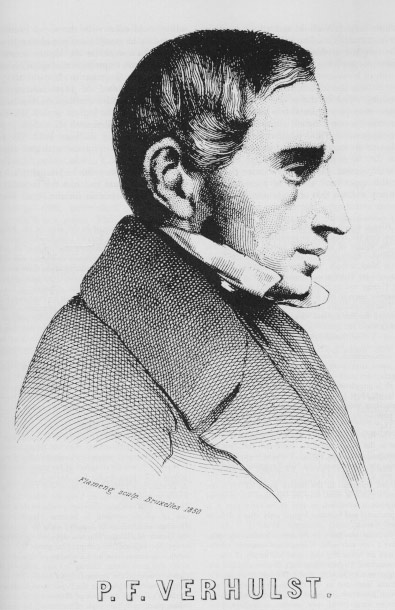
\includegraphics[scale = 0.15]{lesson_1/images/logistic_model_verhulst.jpg}
    \hspace{1em}
    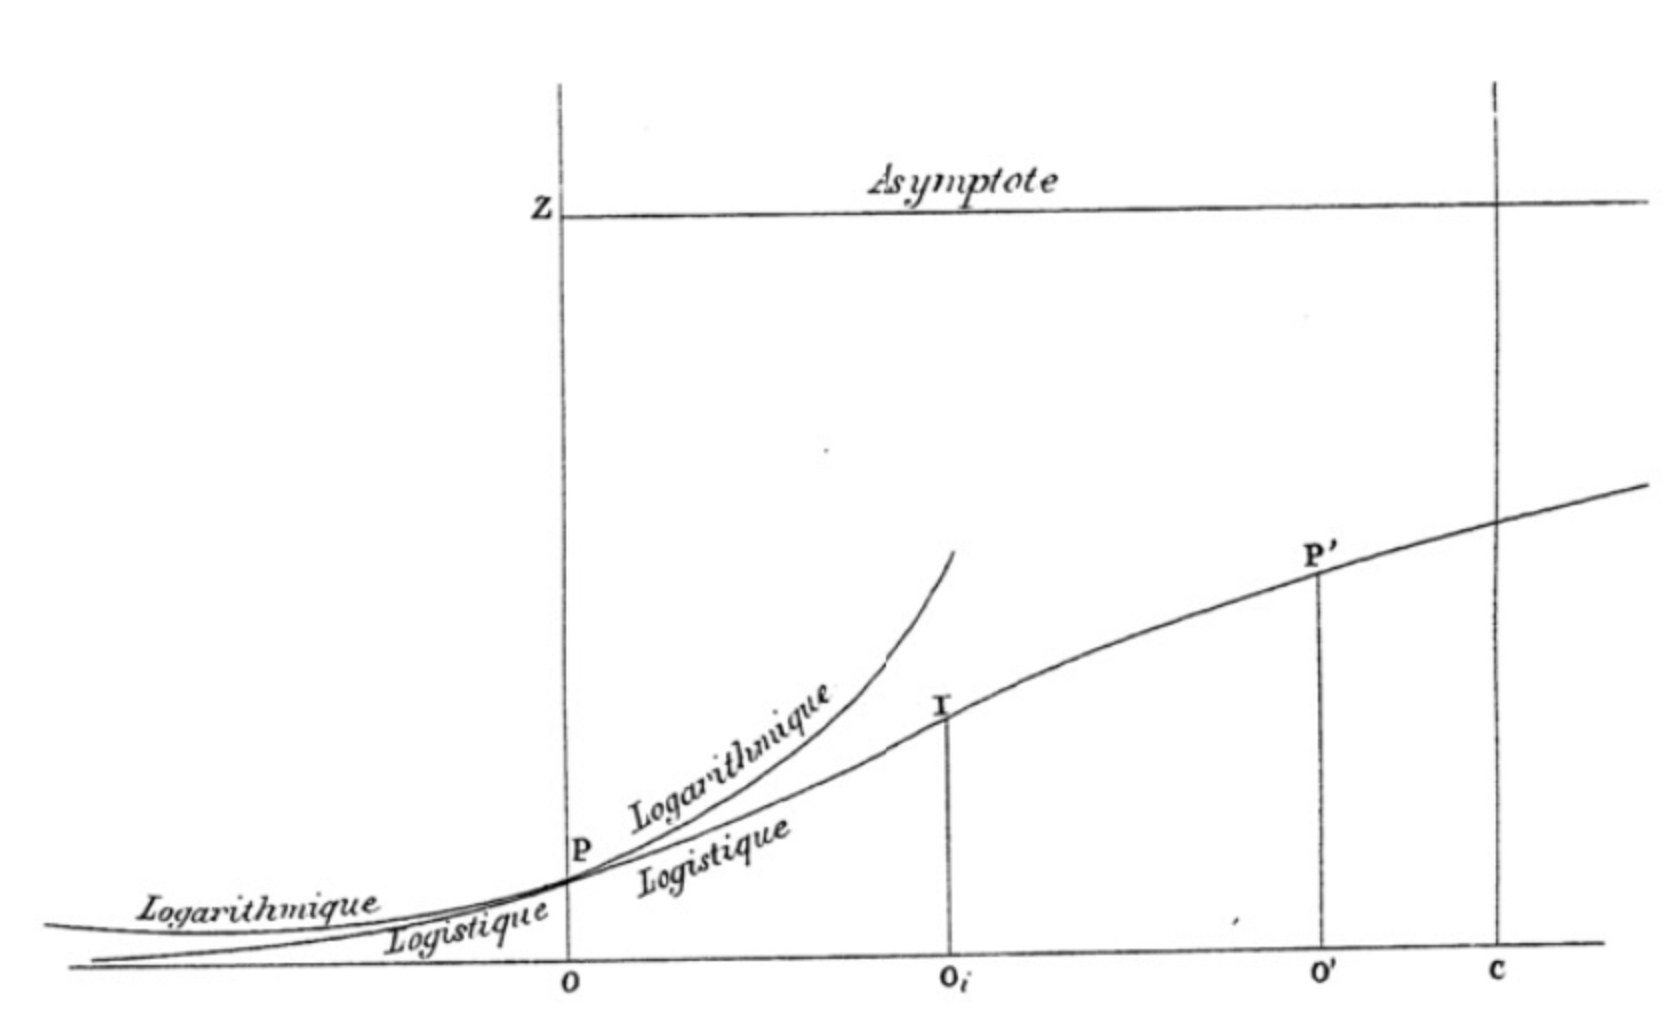
\includegraphics[scale = 0.2]{lesson_1/images/logistic_model_historical.png}
           \textit{Pierre Verhulst and the first plot of logistic growth curve}
    \end{center}
\end{frame}

\begin{frame}{The logistic growth model has extensive applications}

\begin{itemize}
    \item \textbf{Biology} : Used extensively in modeling animal, plant and bacterial population growth
    \pause
    \item \textbf{Epidemiology and medicine}: Helps analyze how diseases spread within a population or growth of tumor.
    \pause
    \item \textbf{Economics}: Model of market adoption of new products or technologies --- a diffusion of innovation
    \pause
    \item \textbf{Linguistics}: an innovation that is at first marginal begins to spread more quickly with time, and then more slowly as it becomes more universally adopted.
    \pause
    \item \textbf{Statistics and machine learning} Logistic functions are often used in artificial neural networks to introduce nonlinearity in the model --- but it is mostly for the shape. 
\end{itemize}

\end{frame}

\subsection{Exercise}



\begin{frame}{Tasks overview}
\footnotesize
\begin{enumerate}
    \item Numerically solve the logistic growth equation and plot:
    \begin{itemize}
    \footnotesize
        \item Population size vs time
        \item Population increase vs time
        \item Per capita growth rate vs population size
        \item Population increase vs population size
    \end{itemize}
    \pause
    \item Adjust the appearance of the plot
    \begin{itemize}
    \footnotesize
        \item Add plot title and axis labels 
        \item Change line thickness and appearance
        \item Experiment with other changes.
    \end{itemize}
    \pause
    \item Experiment with model parameters
        \begin{itemize}
        \footnotesize
            \item Try to increase the initial population over the capacity of the environment
        \end{itemize}
    \item Model the population\textsuperscript{*} of the USA and compare it with real data.
\end{enumerate}

\tiny
\textsuperscript{*}\textit{For the population model of the USA, set step size to 1 month, the initial population size to 5.2 million in 1790,the growth rate to 0.0237, and the capacity of the environment to 460 million.}
\end{frame}

\begin{frame}[fragile]{Solution 3.1: Logistic growth model} 
\only<1>{
\tiny
\vfill
\lstinputlisting
{lesson_1/code/task_3_1_logistic_growth.m}
}
\only<2>{
\begin{center}
   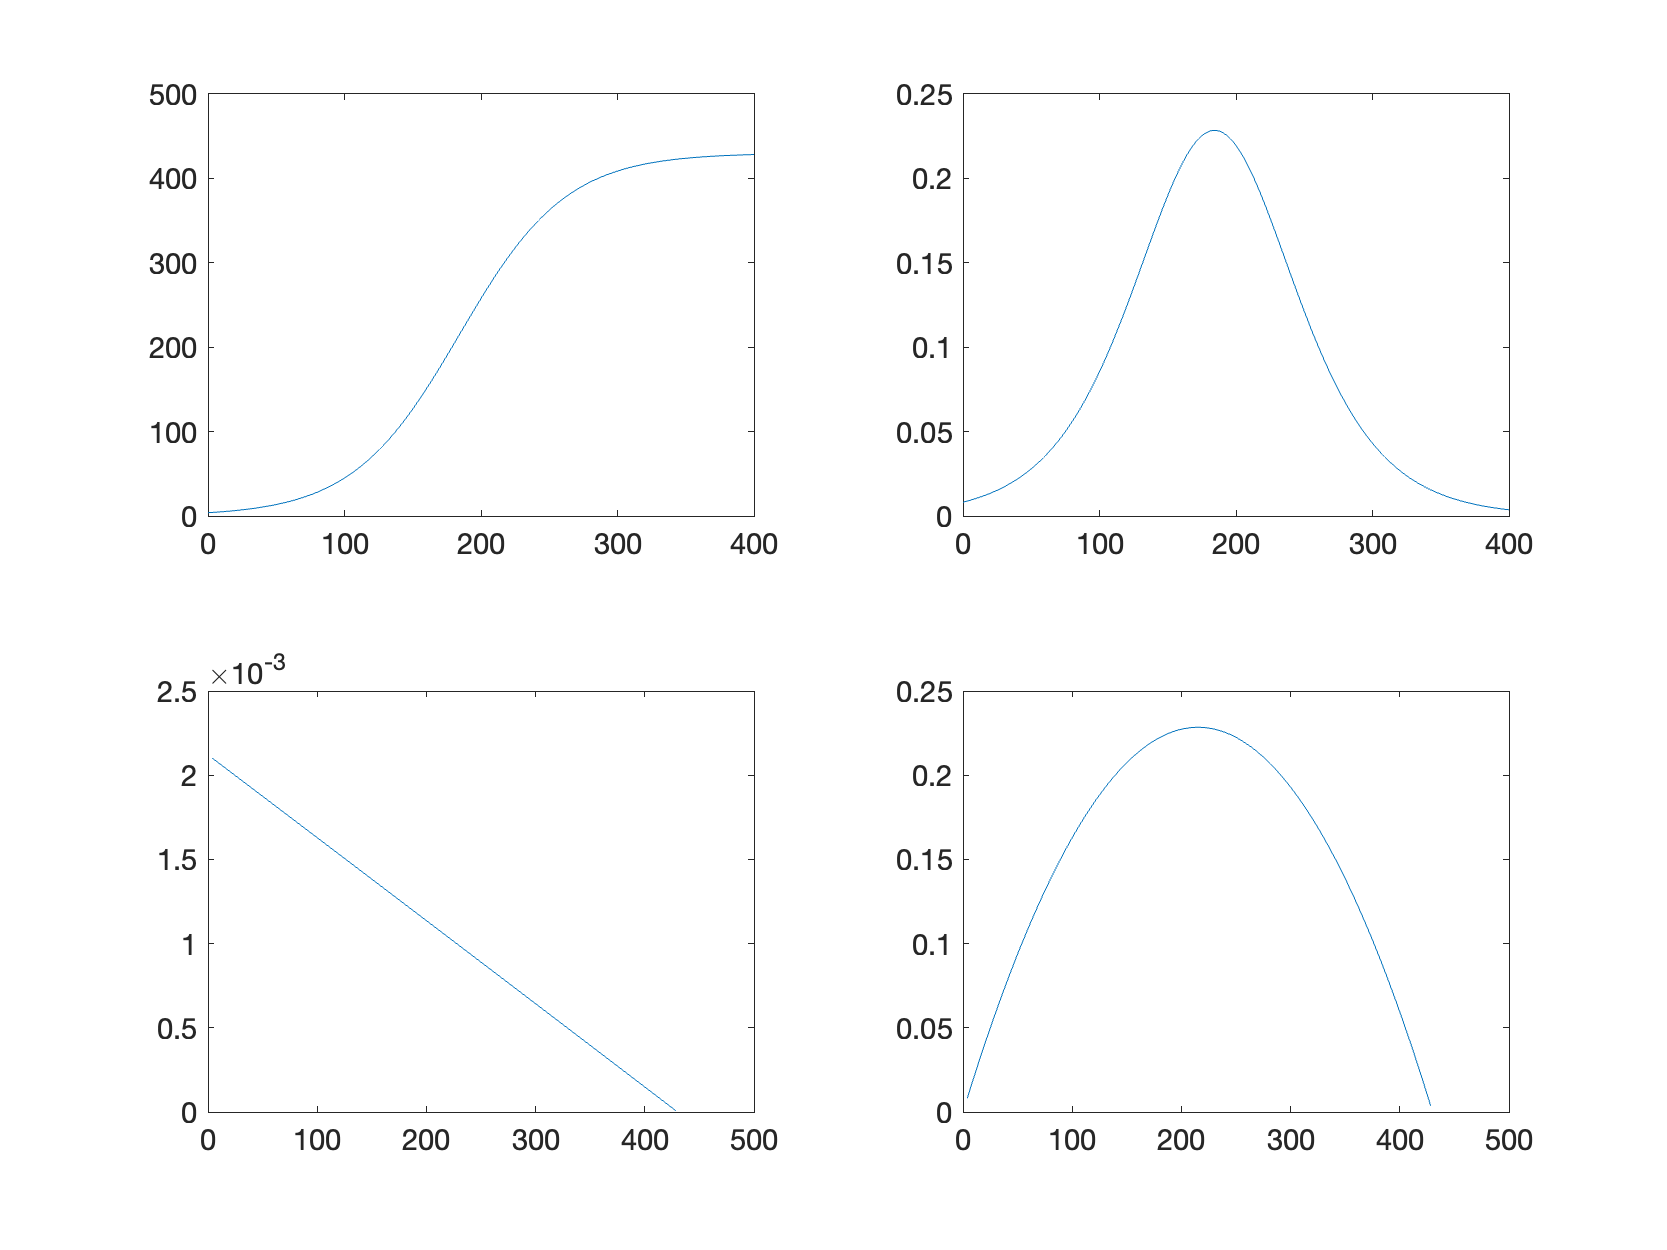
\includegraphics[scale = 0.35]{lesson_1/images/task_3_1_logistic_growth.png}  
\end{center}
}
\end{frame}

\begin{frame}[fragile]{Solution 3.2: Adjusted plot} 
\only<1>{
\vfill
\tiny
\lstinputlisting
{lesson_1/code/task_3_2_logistic_growth_plot.m}
}
\only<2>{
\begin{center}
    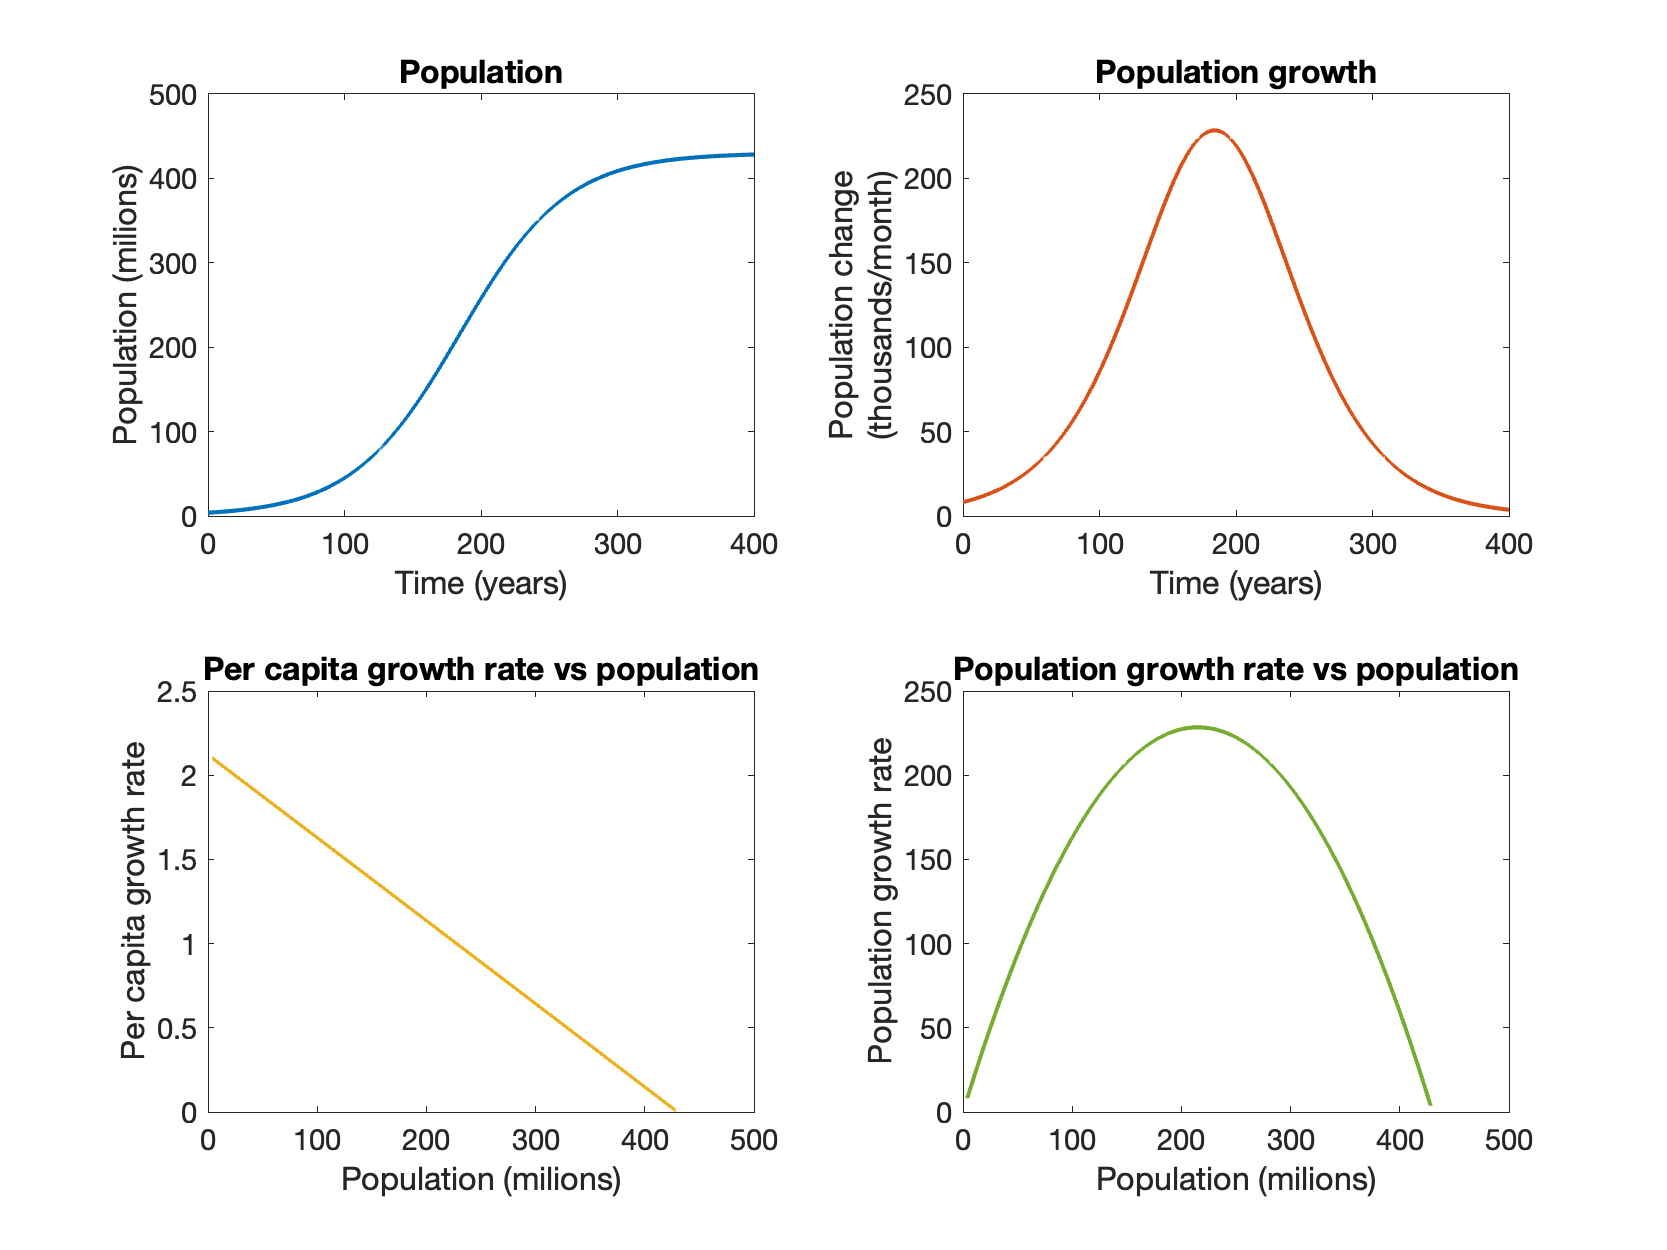
\includegraphics[scale = 0.35]{lesson_1/images/task_3_2_logistic_growth.png} 
\end{center}

}
\end{frame}

\begin{frame}[fragile]{Solution 3.3: US population}
\only<1>{
\vfill
\tiny
\lstinputlisting
{lesson_1/code/task_3_3_logistic_growth_usa.m}
}
\only<2>{
\begin{center}
    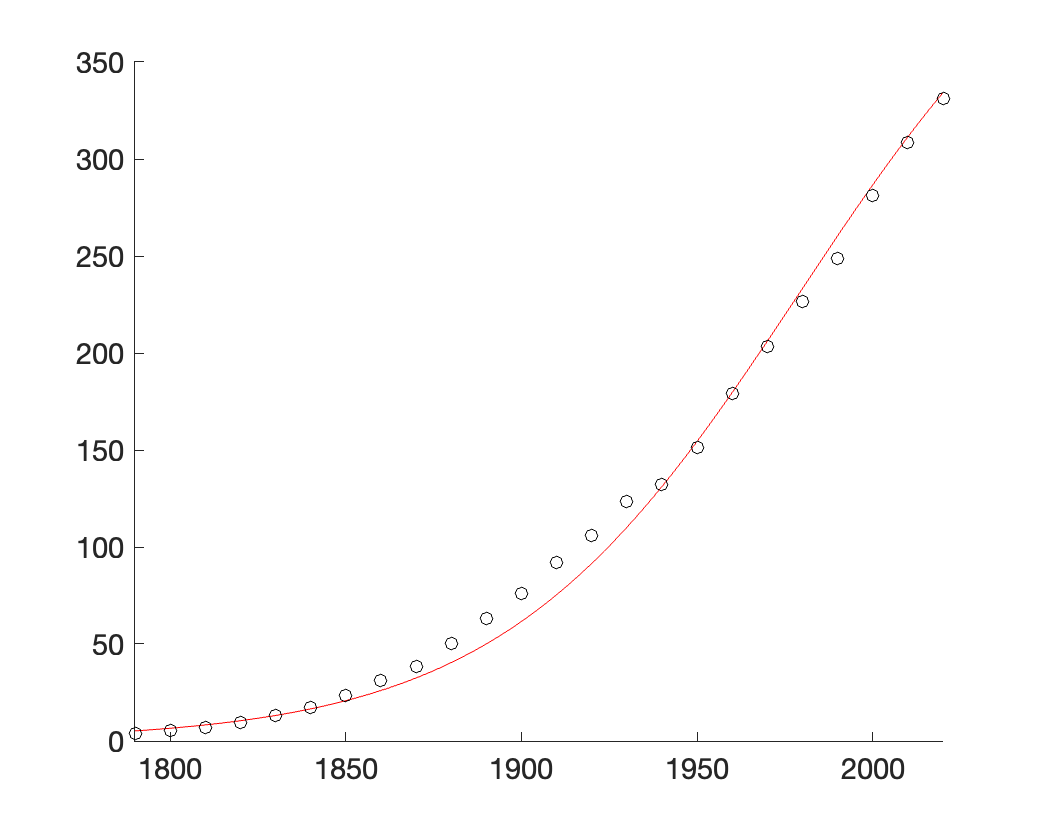
\includegraphics[scale = 0.35]{lesson_1/images/task_3_3_logistic_usa.png} 
\end{center}

}
\end{frame}

